\section{Charged Jets Analysis}

\subsection{Inclusive jets reconstruction}

In this work, the charged jets are obtained by the strategy used
in~\cite{Ali2013:ana933}.
The signal jets are reconstructed by the following criteria:
\begin{itemize}
\item charged track selection:
      \begin{itemize}
      \item acceptance: $\pT>0.15~\GeVc$ and $|\eta|<0.9$ (TPC acceptance),
      \item hybrid track filter: the same as the that used in Pb--Pb
            collision taken in 2011;
      \end{itemize}
\item jet reconstruction:
      \begin{itemize}
      \item jet finder: anti-$\kT$, $R_{\rm jet}=0.4,~0.3$ and $0.2$,
      \item acceptance: $|\eta|<0.5$.
      \end{itemize}
\end{itemize}

\subsection{Jet background density}

The jet background density~\cite{Cacciari:2007fd,Cacciari:2008gn}
is estimated by the jet constituents reconstructed by $\kT$ algorithm with the
same track and acceptance cuts as the signal jets.
To minimize the local track density fluctuations in p--Pb collisions,
a method derived from the so called CMS method~\cite{Chatrchyan:2012tt} (see
also~\cite{Ali2013:ana933} for the implementation in ALICE) is adopted
in this analysis.
This method includes the following steps:
\begin{itemize}
\item calculate the jet backgrond density with $\kT$-jets according to the
      median approach~\cite{Cacciari:2007fd}:
      \begin{equation}\label{eq:c04defineRhoBkg}
      \rho_{\rm bkg}={\rm median}\{\frac{\pT^{\rm jet}}{A_{\rm jet}}\};
      \end{equation}
      where, $A_{\rm jet}$ is the jet area defined in~\cite{Cacciari:2008gn};
\item scale $\rho_{\rm bkg}$ with the ratio between the area covered by jets
      and the event acceptance in $\eta-\phi$ plane:
      \begin{equation}\label{eq:c04defineRhoCMS}
      \rho_{\rm CMS}=\frac{\rm area~covered~by~jets}{\rm total~area}
                     \rho_{\rm bkg};
      \end{equation}
\item to further refined the CMS method in p--Pb collisions,
      the $\kT$-jets that share tracks with the signal jets (anti-$\kT$ jets)
      are removed in the calculation of the background density in
      eq.~(\ref{eq:c04defineRhoBkg}) and the area scale factor
      in eq.~(\ref{eq:c04defineRhoCMS}).
\end{itemize}

\begin{figure}[htb]
\begin{center}
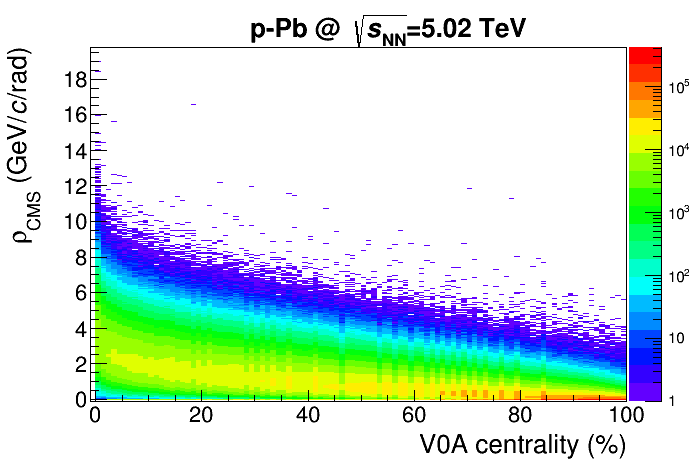
\includegraphics[width=.48\textwidth]{cJetRhoCent}
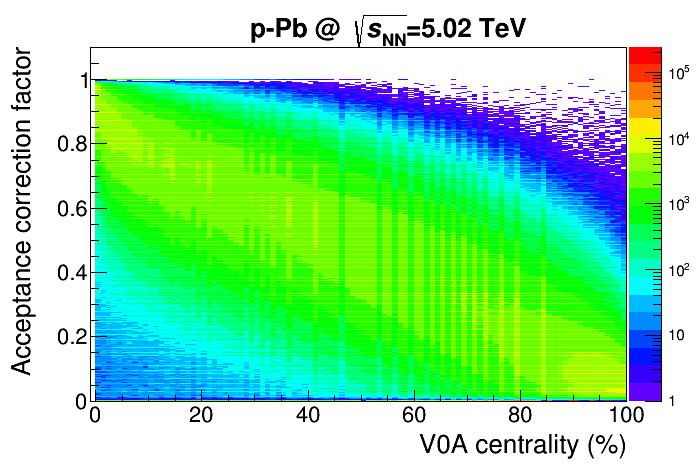
\includegraphics[width=.48\textwidth]{cJetAccCorr}
\caption{Left: 2D distribution of $\rho_{\rm CMS}$ vs. event multiplicity;
         right: 2D distribution of the acceptance correction factor vs.
         event multiplicity.
         The centrality estimator is V0A.}
\label{fig:c04BkgRhoCent}
\end{center}
\end{figure}

Figure~\ref{fig:c04BkgRhoCent} shows
the 2D distributions of $\rho_{\rm CMS}$ vs. event multiplicity (left)
and acceptance correction factor vs. event multiplicity (right).
The centrality estimator is V0A.
As expected, both the jet background density and the acceptance correction
factor decreases with the event multiplicity.

\begin{figure}[htb]
\begin{center}
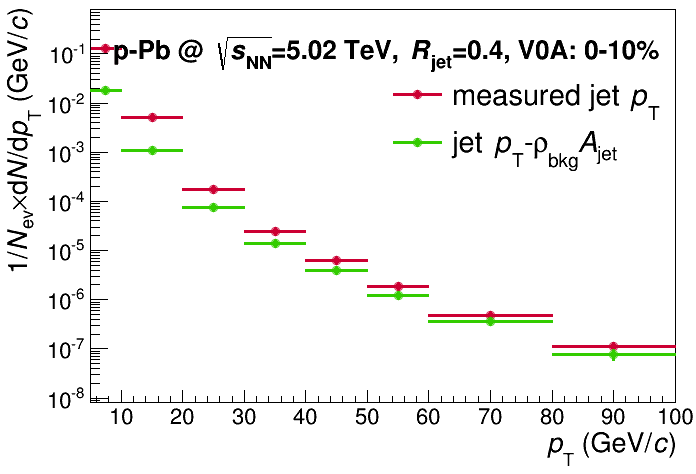
\includegraphics[width=.32\textwidth]{cComp_EstiJetPtR04_V0A_0}
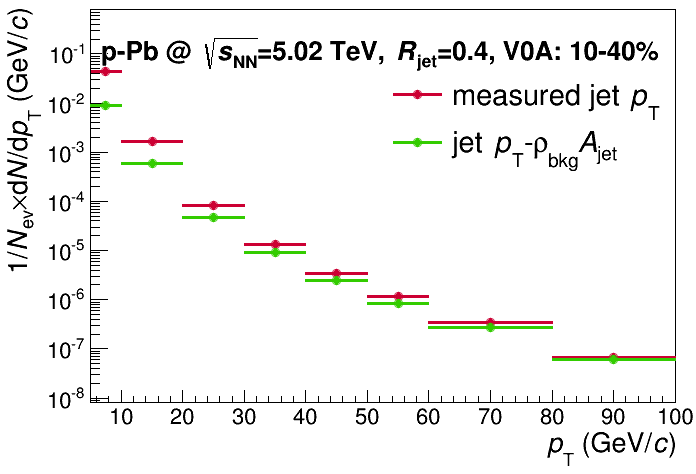
\includegraphics[width=.32\textwidth]{cComp_EstiJetPtR04_V0A_1}
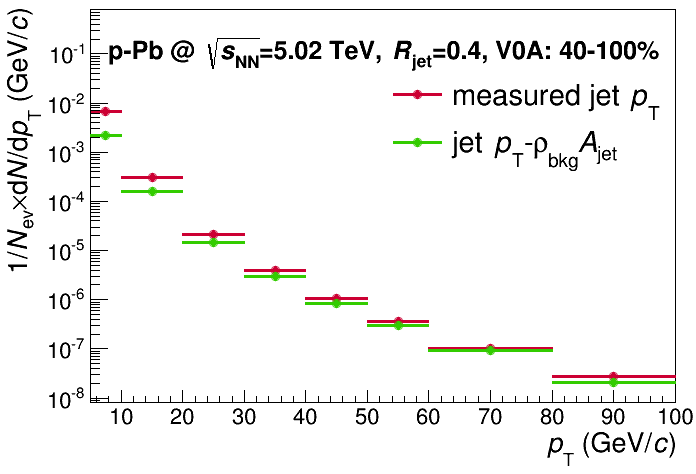
\includegraphics[width=.32\textwidth]{cComp_EstiJetPtR04_V0A_2}
\caption{The comparison of measured jet $\pT$ spectrum and the corrected
         jet $\pT$ spectrum in three event multiplicity bins
         with V0A estimator.
         The jets are measured with $R_{\rm jet}=0.4$.}
\label{fig:c04EstiJetPtR04V0A}
\end{center}
\end{figure}

\begin{figure}[htb]
\begin{center}
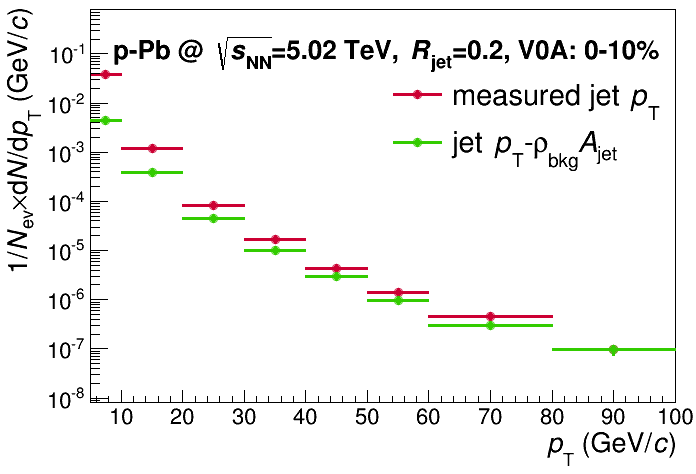
\includegraphics[width=.32\textwidth]{cComp_EstiJetPtR02_V0A_0}
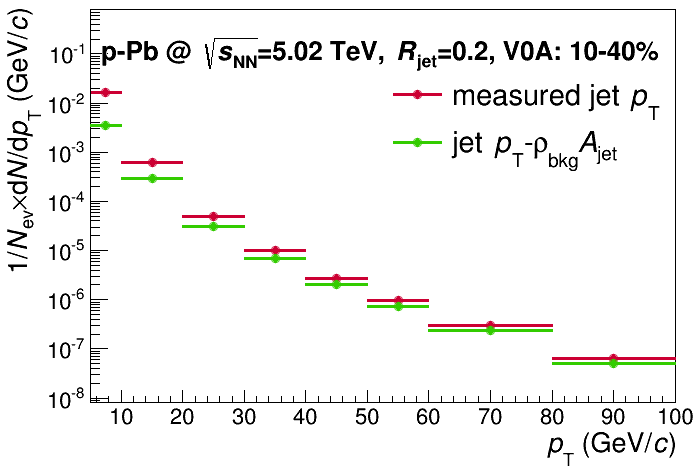
\includegraphics[width=.32\textwidth]{cComp_EstiJetPtR02_V0A_1}
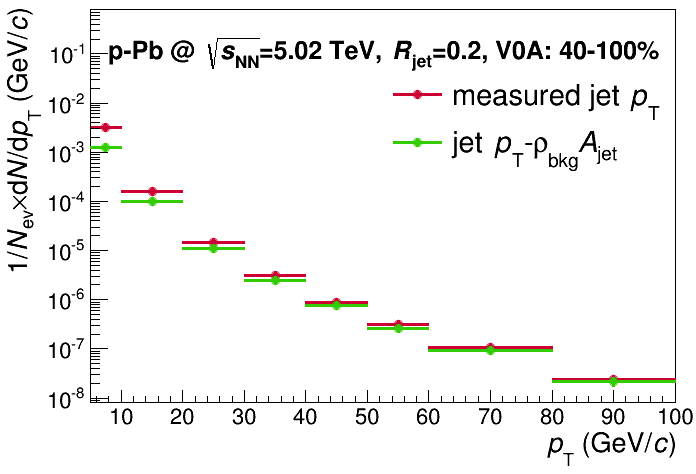
\includegraphics[width=.32\textwidth]{cComp_EstiJetPtR02_V0A_2}
\caption{The comparison of measured jet $\pT$ spectrum and the corrected
         jet $\pT$ spectrum in three event multiplicity bins
         with V0A estimator.
         The jets are measured with $R_{\rm jet}=0.2$.}
\label{fig:c04EstiJetPtR02V0A}
\end{center}
\end{figure}

After obtaining the jet background density,
the estimated jet $\pT$ is given by correcting the measured jet $\pT$
with the background:
\begin{equation}\label{eq:c04DefEstiJetPT}
\pT^{\rm esti}=\pT{\rm meas}-\rho\cdot A_{\rm jet},
\end{equation}
where, $\pT^{\rm meas}$ is the measured jet $\pT$ and $A_{\rm jet}$ is the jet
area, jet background density is given by the $\rho_{\rm CMS}$
in eq.~(\ref{eq:c04defineRhoCMS}).

The measured jet $\pT$ spectrum and the estimated jet $\pT$ spectrum in three
event multiplicity bins are compared in
figure~\ref{fig:c04EstiJetPtR04V0A} (with $R_{\rm jet}=0.4$)
and figure~\ref{fig:c04EstiJetPtR02V0A} (with $R_{\rm jet}=0.2$),
respectively.
The discrepancy between them decreases when jet $\pT$ increasing.

\begin{figure}[htb]
\begin{center}
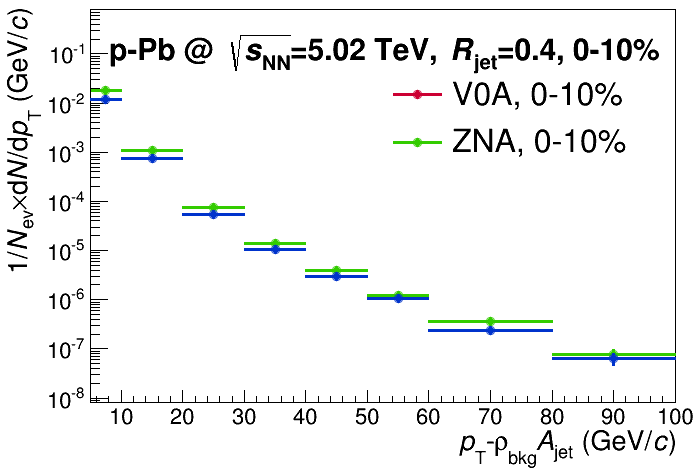
\includegraphics[width=.32\textwidth]{cComp_EstiJetPtR04_ZNA_0}
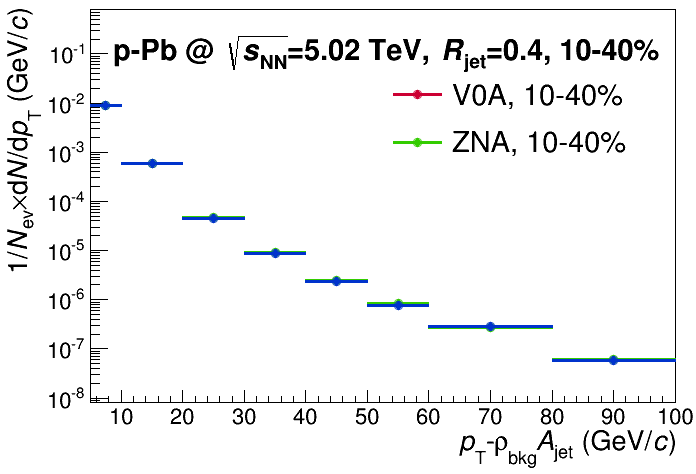
\includegraphics[width=.32\textwidth]{cComp_EstiJetPtR04_ZNA_1}
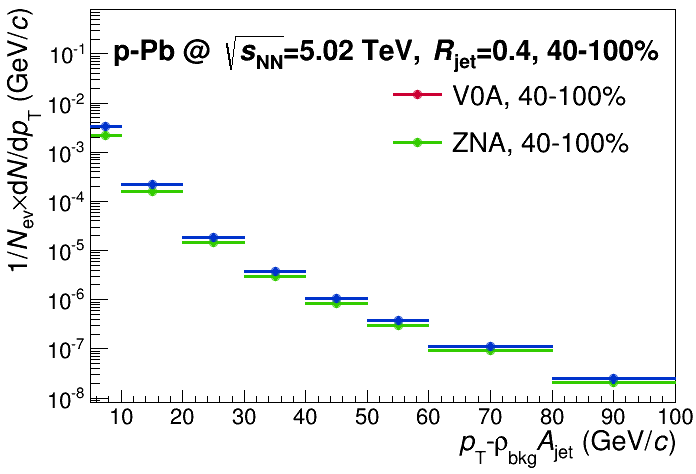
\includegraphics[width=.32\textwidth]{cComp_EstiJetPtR04_ZNA_2}
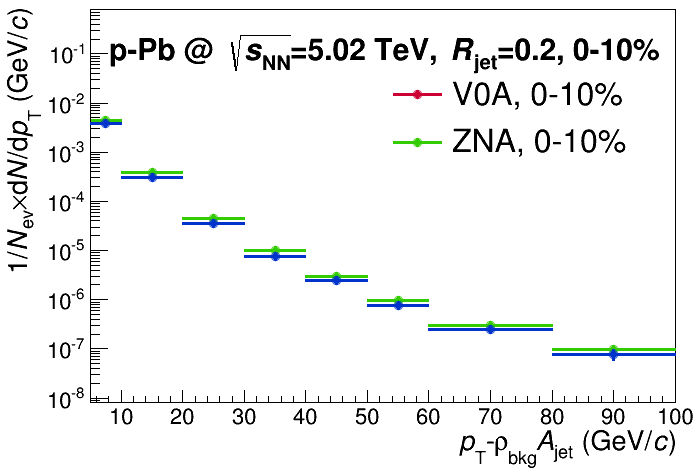
\includegraphics[width=.32\textwidth]{cComp_EstiJetPtR02_ZNA_0}
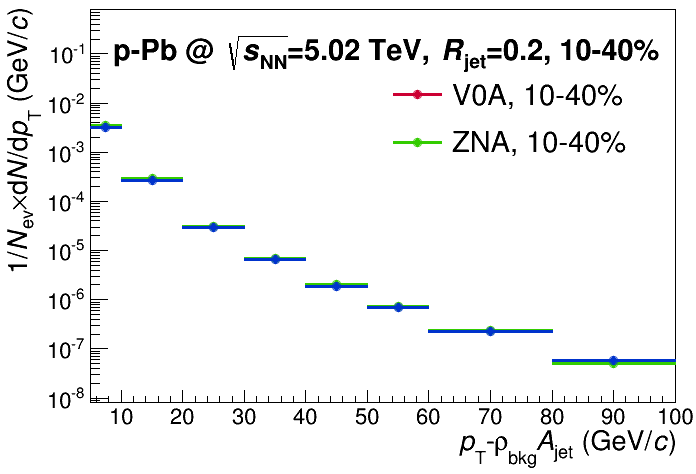
\includegraphics[width=.32\textwidth]{cComp_EstiJetPtR02_ZNA_1}
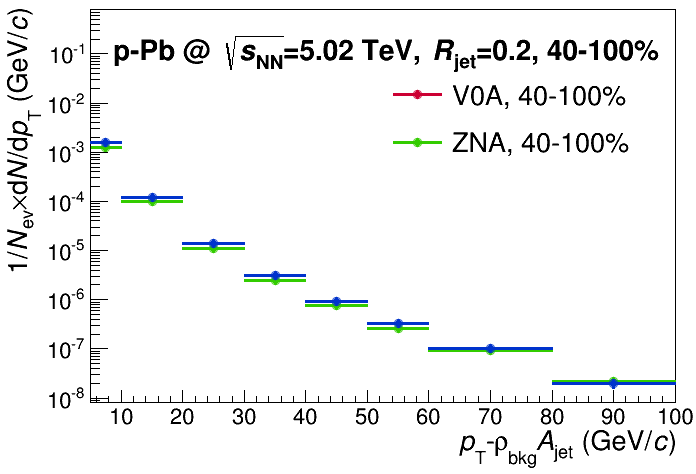
\includegraphics[width=.32\textwidth]{cComp_EstiJetPtR02_ZNA_2}
\caption{The comparison of corrected jet $\pT$ spectra obtained with the V0A
         centrality estimator and those obtained with the ZNA centrality
         estimator in three event multiplicity bins.
         The jets are measured with $R_{\rm jet}=0.4$ (upper)
         and $R_{\rm jet}=0.2$ (lower).}
\label{fig:c04EstiJetPtZNA}
\end{center}
\end{figure}

Due to the acceptance of the V0A ($2.8<\eta<5.1$) is closer to the jet
acceptance (the jet constituents are selected in $|\eta|<0.9$) and it has the
correlations between the reconstructed jets at the mid-rapidity.
To decrease the acceptance correlations as well as to study the systematic
uncertainty on different centrality estimators,
the ZNA ($|\eta|\sim 8$) is also used in this analysis.
Figure~\ref{fig:c04EstiJetPtZNA} shows the comparison of corrected
jet $\pT$ spectra obtained with the V0A centrality estimator and those obtained
with the ZNA centrality estimator in three event multiplicity bins.
The results with $R_{\rm jet}=0.4$ are presented in the upper three plots and
the results with $R_{\rm jet}=0.2$ are presented in the lower three plots.
The discrepancy between the two centrality estimators is visible in the
central ($0-10\%$) and peripheral ($40-80\%$) collisions and they give almost
the some results in the semi-central collisions ($10-40\%$).

\subsection{Background fluctuations}

The fluctuations of jet background density,
which illustrated by the observable $\delta\pT$,
is evaluated by using the random cone method~\cite{Abelev:2012ej}.
The approaches are:
\begin{itemize}
\item throw the cones with same radius as the jet and randomized
      $\eta$ and $\phi$ in the jet acceptance in each event;
\item calculate the $\delta\pT$:
      \begin{equation}
      \delta\pT=\sum_{\rm in~cone}\pT-\rho\cdot A_{\rm cone},
      \end{equation}
      where, the sum runs the selected tracks in the cone,
      $A_{\rm cone}=\pi R_{\rm jet}^{2}$ is the cone size.
      The $\rho_{\rm CMS}$ is used in calculation in this analysis.
\end{itemize}
With this definition, the non-zero value of $\delta\pT$ shows the
difference between the track $\pT$ that in a random chosen and
the expected background of jets.
Statistically, it gives the fluctuations of the background.
Another source for non-zero $\delta\pT$ given by the cone can overlap with
the jets.
It is not problematic since jets can also overlap each other.
To account for this, in the calculation of the $\delta\pT$,
the random cones overlapping with the leading jet is rejected with a
probability given by:
\begin{equation}
p=\frac{1}{N_{\rm coll}},
\end{equation}
where $N_{\rm col}$ is the average number of hard collisions per
minimum bias event.
With the partial exclusion, $R_{\rm pPb}$ of charged jets is changed by less
than $1\%$~\cite{Ali2013:ana933}.
Figure~\ref{fig:c04DeltapT} shows the $\delta\pT$ distribution
in this analysis,
the RMS of this distribution is $\sim 1~\GeVc$.

\begin{figure}[htb]
\begin{center}
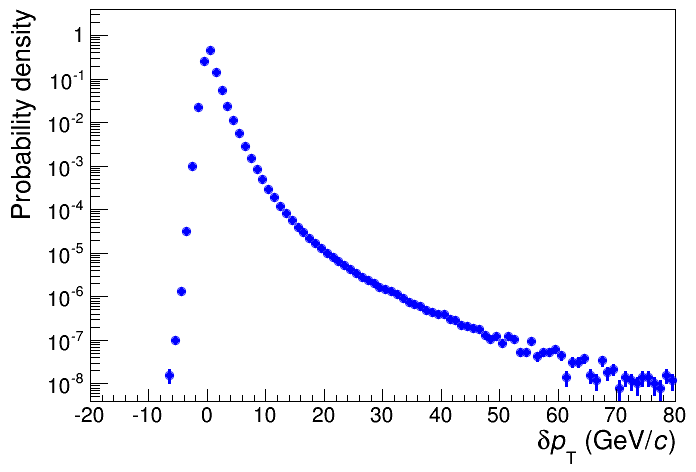
\includegraphics[width=.8\textwidth]{cLHC13bR04_SVD_DeltaPt}
\caption{The $\delta\pT$ distribution obtained by the random cone approach
         with the $\rho_{\rm CMS}$.}
\label{fig:c04DeltapT}
\end{center}
\end{figure}

\subsection{Detector response matrix}

The single track efficiency and resolution also affects the
resolution of the reconstructed jet $\pT$.
These effects are described by the detector response matrix,
which is built as:
\begin{itemize}
\item simulate events with the realistic detector configurations as
      those in data;
\item run the jet finder at particle level (over the generated particles,
      which have no detector effect);
\item represent the jet finder at the detector level (over the reconstructed
      tracks);
\item match the jets at particle level and detector level with
      $\Delta R<0.1$ in the $\eta-\phi$ plan;
\item the detector response matrix is built as the correlations of the $\pT$
      for jets at particle level and that at detector level.
\end{itemize}

\begin{figure}[htb]
\begin{center}
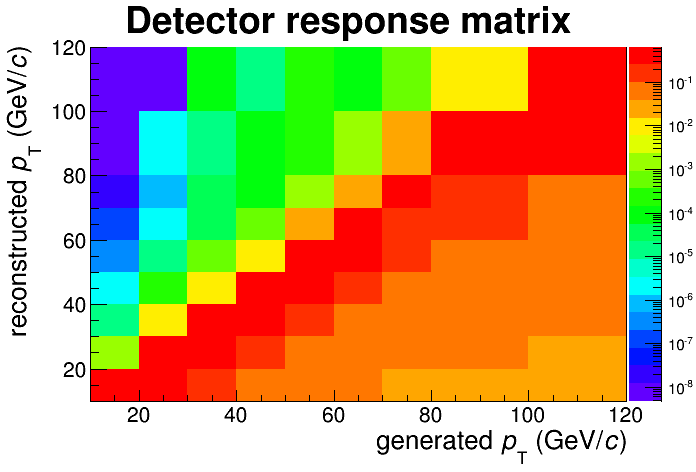
\includegraphics[width=.8\textwidth]{cLHC13bR04_SVD_DetectorRM}
\caption{The $\delta\pT$ distribution obtained by the random cone approach
         with the $\rho_{\rm CMS}$.}
\label{fig:c04DetectorRM}
\end{center}
\end{figure}

In this analysis, the detector response matrix is obtained from LHC13b4
simulations which are introduced in section~\ref{sec:03PySampleMC}.
Figure~\ref{fig:c04DetectorRM} shows the detector response matrix used in
this analysis.
